% CREATED BY DAVID FRISK, 2015
\chapter{Theoretical Framework}

\lettrine[findent=2pt]{\fbox{\textbf{T}}}{ }his chapter introduces theory that is related to this study covering the areas of architectures in automotive domain, the two types of electrical architectures at VCG, and the proprietary tool Elektra that stores the low-level architectures. Theory of data collection method is also explained in this chapter. Related works will be discussed through out the chapter.

\section{Architectures in automotive domain}
Proper architecture is necessary for designing and building modern vehicles which mostly are driven by electronics and software. Here are some related works that explain how it plays an important role in automotive domain.\\

Beeck \cite{Beeck} developed a modeling approach for development of software for ECUs at BMW Group, which supports the development of logical and technical architectures (high- and low-level architectures, respectively). The approach was developed based on the notation Unified Modeling Language for Real-Time (UML-RT) to compromise the complexity issue of developing, integrating, and maintaining software-intensive systems in vehicles. The logical architecture model is developed using UML-RT's capsule structure diagrams representing graphical system view of automotive functions. The technical architecture separated into software and hardware architectures is developed using UML-RT's component diagrams (for software) and deployment diagrams (for hardware). \\

For the logical architecture, the author created a UML-RT constructs and used them to model the architecture. From the meta-model (figure \ref{fig:beeck_metalmodel}), capsules, ports, protocols, signals, and connectors notations are used for modeling architectural artifacts. Capsules represent functions, while ports and protocols model function interfaces. A port is used to specify a communication point of a capsule. Each port has associated protocol, which contains two sets of signals: export and import. Connectors represent channels between function interfaces. \\

For the technical architectures, Components are used to model software components. Hardware components such as ECUs and sensors are modelled using UML-RT nodes. \\

The author, however, finds that still there are some issues regarding the use of UML-RT. One of the problems is, the set of UML-RT diagram notations is quite restricted. It is hard for ECU developers, who are familiar with non-object-oriented notations, to work with. In addition, the two protocols associated with ports do not meet requirements of some ECUs.

\begin{figure}[H]
\centering
\captionsetup{justification=centering}
\vspace{0cm}% Adjust vertical spacing here
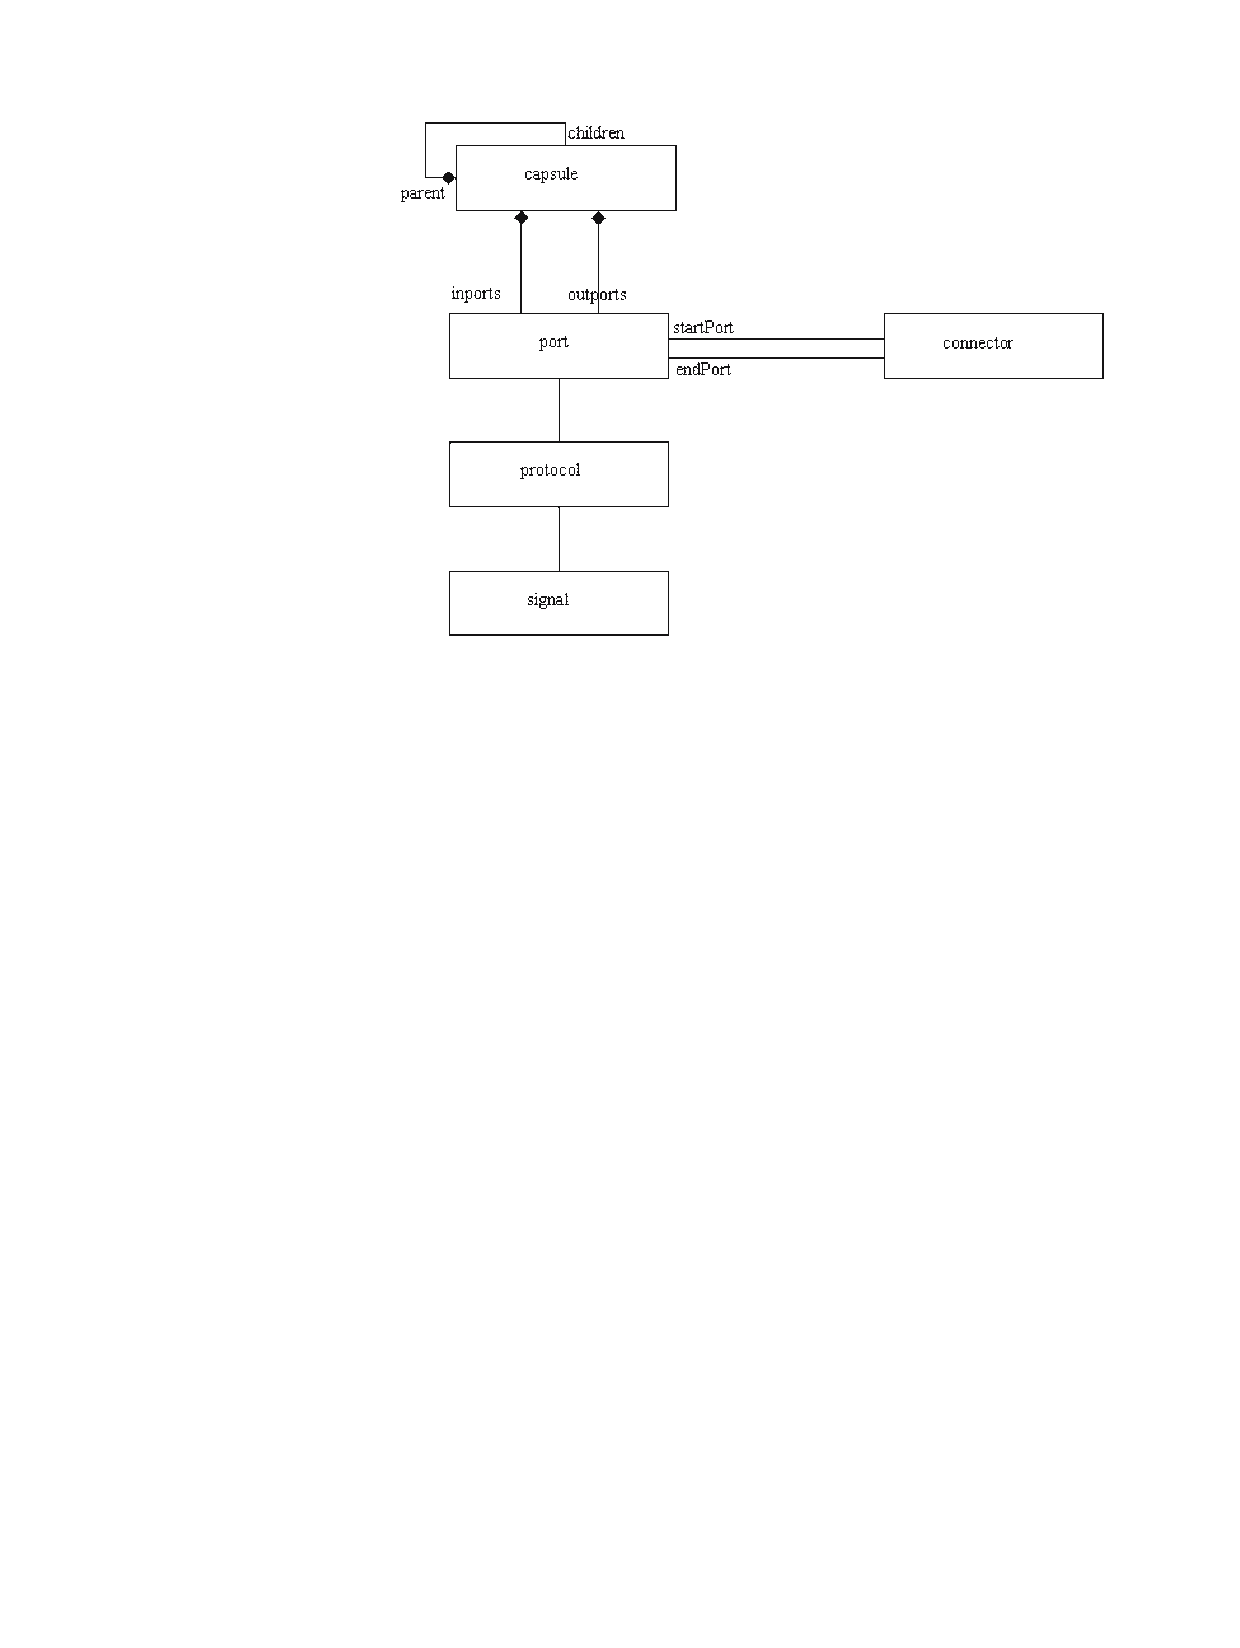
\includegraphics[width=0.55\linewidth]{figure/literatures/beeck_metalmodel.pdf}
\caption{Meta-model of UML-RT constructs for logical architecture \cite{Beeck}}
\label{fig:beeck_metalmodel}
\end{figure}

Grönniger et al. \cite{Grönniger} developed an approach for modelling logical architectures of automotive systems using views. Function nets which are valid Systems Modeling Language (SysML) Internal Block Diagrams (IBD) are used to model complete automotive functions and views which describe the environment and context of a certain aspect of function net. In addition to that, views can be used to model features in a self-contained way, and specify consistency conditions for consistency between a view and a function net.

\begin{figure}[H]
\centering
\captionsetup{justification=centering}
\vspace{0cm}% Adjust vertical spacing here
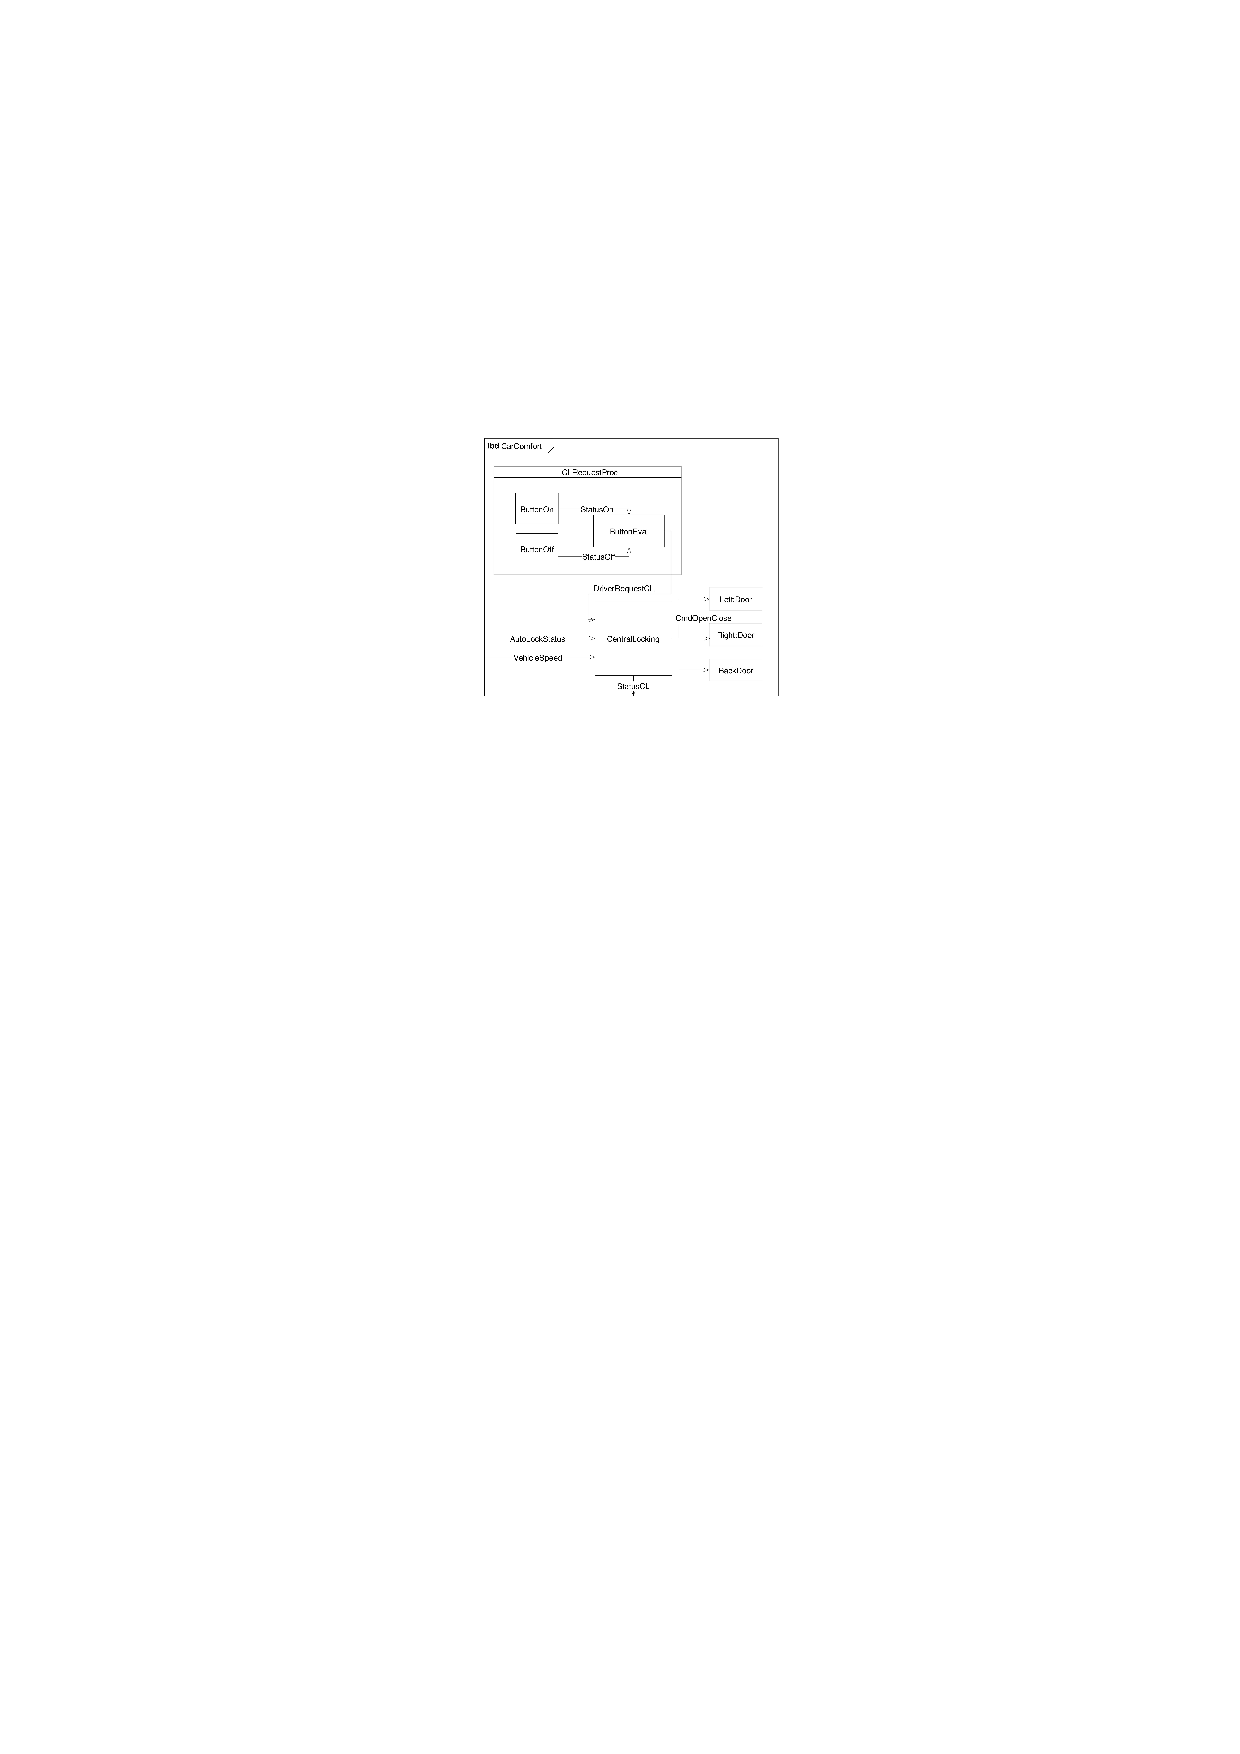
\includegraphics[width=0.35\linewidth]{figure/literatures/gronniger_sysml1.pdf}
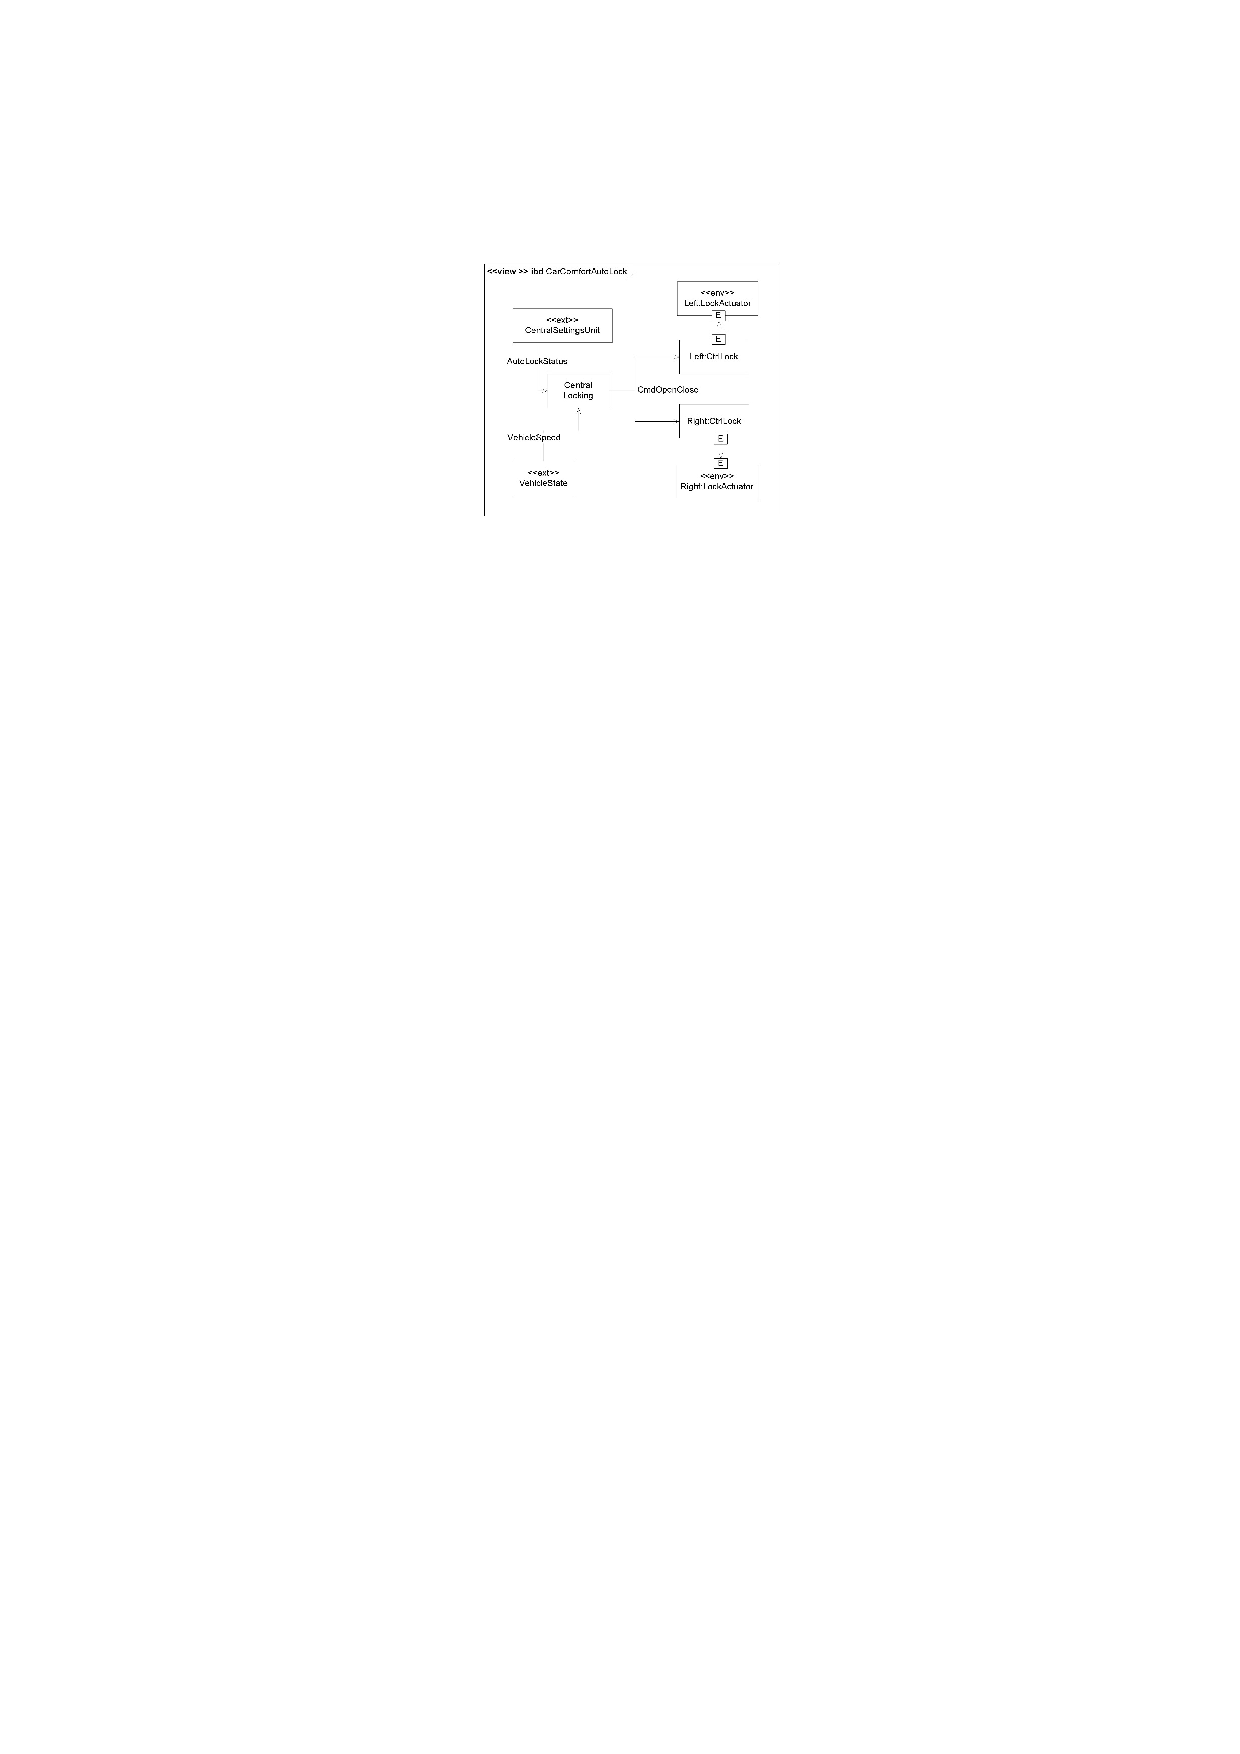
\includegraphics[width=0.35\linewidth]{figure/literatures/gronniger_sysml2.pdf}
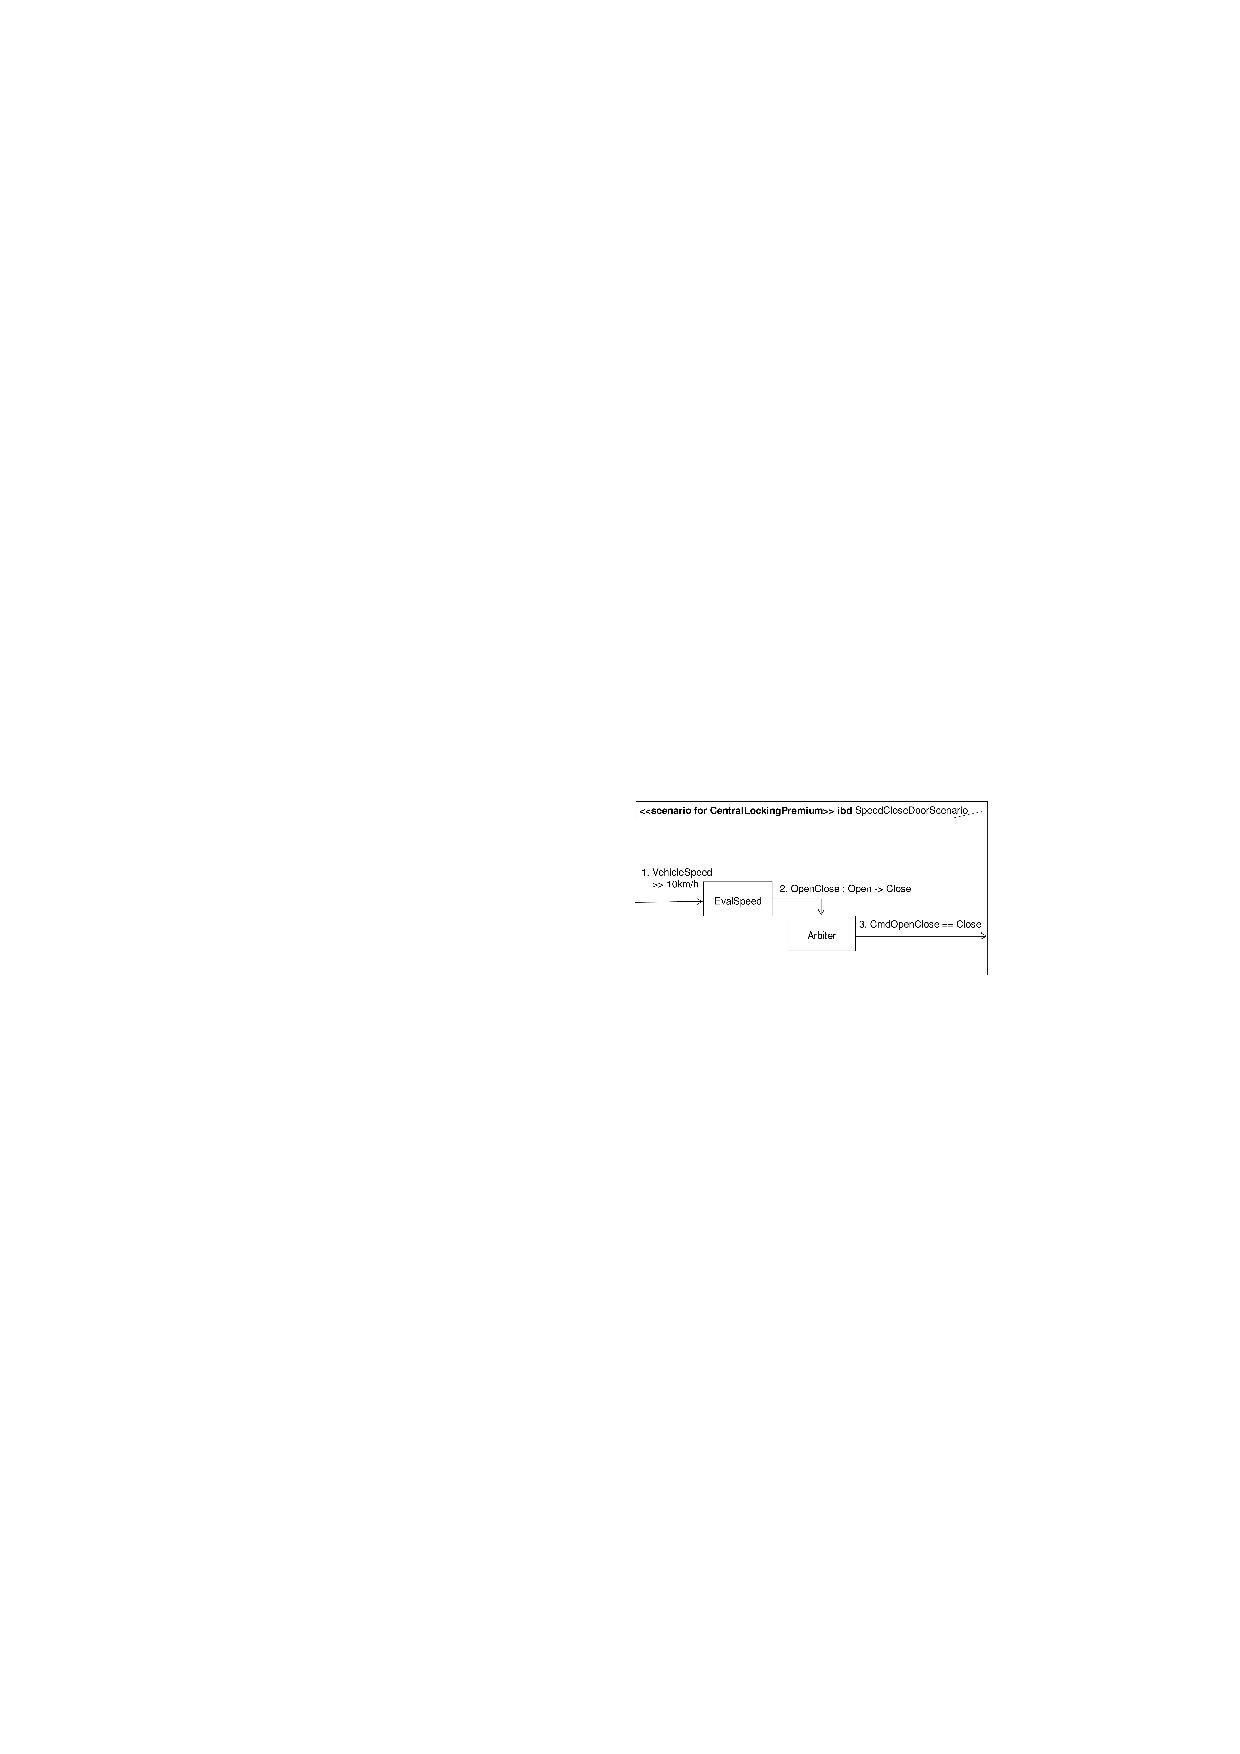
\includegraphics[width=0.5\linewidth]{figure/literatures/gronniger_sysml3.pdf}
\caption{Examples of a functional net \texttt{CarComfort} (top left), a view \texttt{CarComfortAutoLock} (top right), and a scenario \texttt{SpeedClosedDoorScenario} (bottom) \cite{Grönniger}}
\label{fig:gronniger_sysml}
\end{figure}

The authors claim that function nets and views can be used to describe and explain scenarios of use-cases like how an automotive system reacts to external events or failures caused by subsystems (see figure \ref{fig:gronniger_sysml}). However, number of models have to be created as well as references between these models. The authors states in their work that an investigation of existing model management strategies to handle number of models will be performed in the future.\\

Dajsuren \cite{Dajsuren} presents a research which is part of Hybrid innovations of Trucks and it covers the automotive Architecture Description Language (ADL) and quality of automotive software. This research has a role of identifying a proper ways of developing automotive software. \\

The author suggests that automotive software development enables interaction between different engineering fields such as mechanical engineering, electrical engineering and software engineering. ADL can be said to be an effective way to manage such multi-disciplinary engineering information. It has been defined on this paper as ``one of the approach to formalize the representation of the automotive systems and software architecture''. Examples of ADL used in automotive companies are definition of AML for BMW company, EAST-ADL and TADL for Volvo, Fiat, and VW/Carmeq. \\

\begin{figure}[H]
\centering
\captionsetup{justification=centering}
\vspace{0cm}% Adjust vertical spacing here
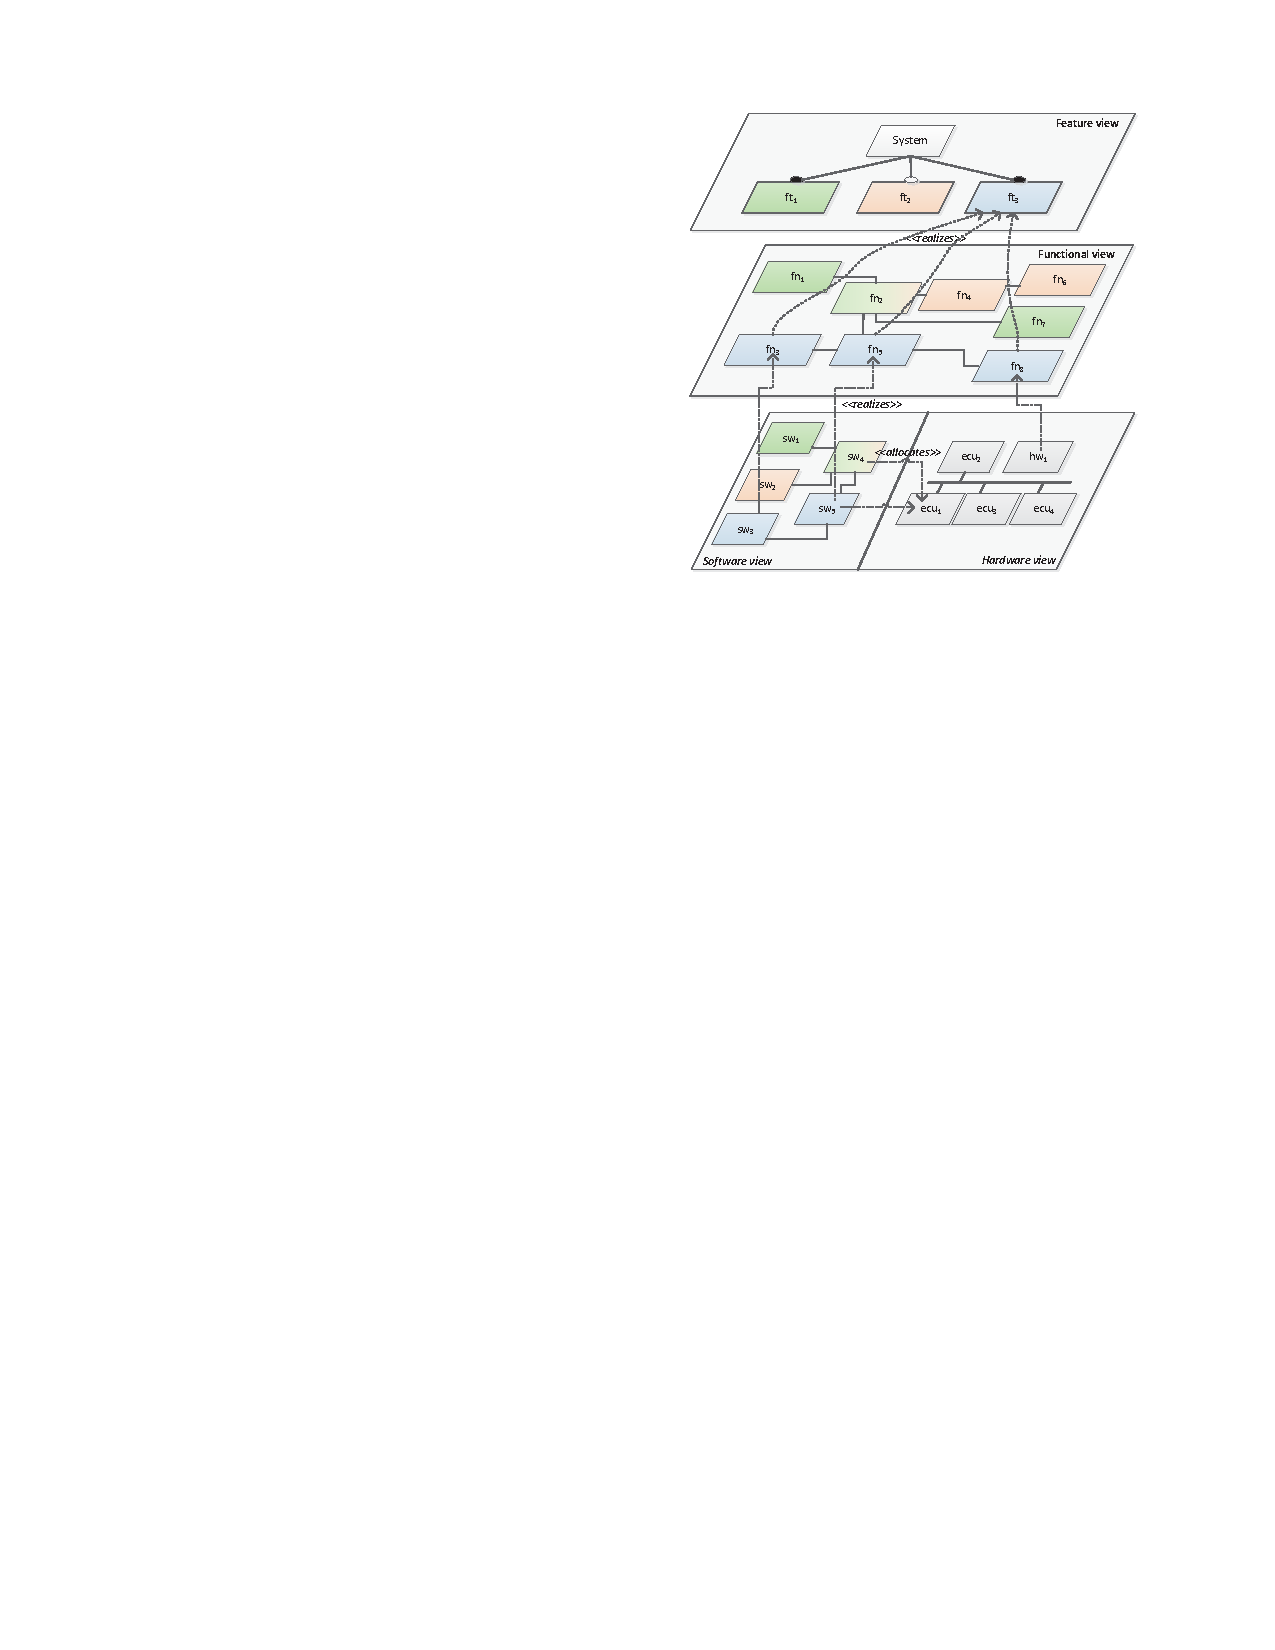
\includegraphics[width=0.5\linewidth]{figure/literatures/dajsuren_adl.pdf}
\caption{Architectural views of an automotive system \cite{Dajsuren}}
\label{fig:dajsuren_adl}
\end{figure}

The different levels of the architecture have been mentioned as well, these include:
\begin{itemize}
    \item \textit{Feature view} that shows number of features in a system.
    \item \textit{Function view} that shows a number of functions or subsystems in a system. A single feature could include one or more function.
    \item \textit{Software view} that shows a detailed architecture. It shows components and blocks which represent the implementation of the functions specified in the function view.
    \item \textit{Hardware view} that contains ECUs, sensors, actuators and Controller Area Network (CAN).
\end{itemize}
\vspace{0.2cm}
The author decided to use and ADL language SysML\footnote{\url{https://sysml.org}} in modelling a functional architecture (view) and MATLAB/Simulink has also been mentioned as one of the most popular graphical modelling language and a simulation tool for modelling software architecture (view). \\

The inconsistency of architecture in multiple views has also been explained. This is one of the problem that VCG also experiences which is in between the high- and low-level architectures. In this paper, a consistency rule has been proposed between the different views of the architecture.\\



\section{Low- and high-level electrical architectures at VCG}
To have a better understanding of how low- and high-level electrical architectures have been constructed and used in VCG. The team studied some related works that were conducted in the company.\\

Eliasson et al. \cite{Eliasson_1} find that VCG and Volvo Group Truck Technology (VGTT) have two types of architectures: a high-level architecture and a working architecture (low-level architecture). The high-level architectures produced by high-level architects contain design decision, principles, rules, and pattern that should govern the overall system. The working architecture produced by low-level architects contains logical components which are broken down from the high-level architecture and more details. The study describes that the working architecture is always kept updated by developers as the product evolve, while the high-level architecture is only updated when the project has started. Because of this reason, the inconsistency between the two architecture occurs. It also suggests that having two different groups of architects results to problems. High-level architects have a thought that the low-level architects are very focused on short-term solutions which make them miss an overall picture of the system, while low-level architects see that another group lacks of understanding of current situation and is too focused on solutions that might be good in long run. \\

From another related work, Eliasson et al. \cite{Eliasson_2} also suggest that the presence of the Architecture Technical Debt (ATD) at the design level at VCG plays an important role on the efficiency of communication between components. In this paper, there is a discovery of the ATD items (architectural violations) such as the misplaced LCs and their impacts on the software development process (see figure \ref{fig:eliasson_atd}). The ATD items together with the inputs from the stakeholders at VCG were used to assist in creating a visual tool which provides a better visualization of the ATD items and its interest. With this tool, the visualization is more comprehensive to the stakeholders. 

%FIGURE
\begin{figure}[H]
\centering
\captionsetup{justification=centering}
\vspace{0cm}% Adjust vertical spacing here
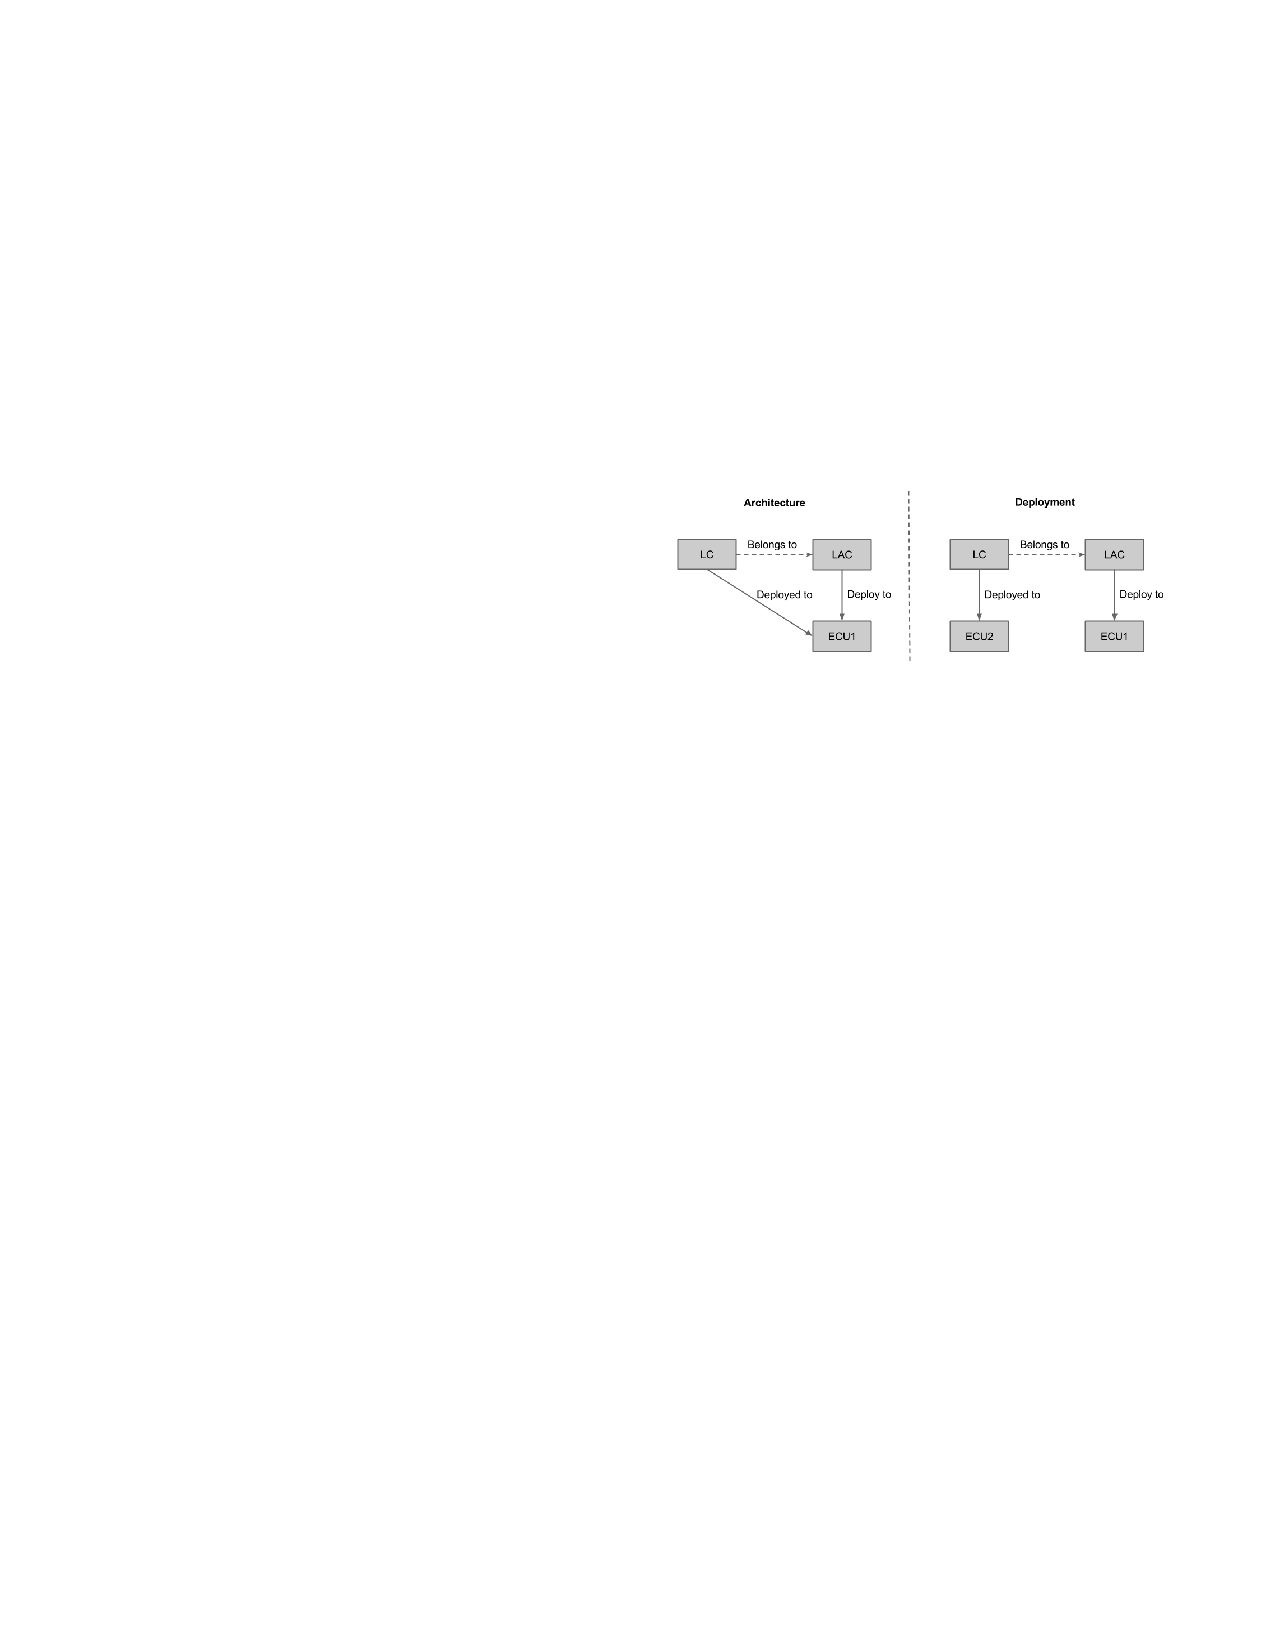
\includegraphics[width=0.7\linewidth]{figure/literatures/eliasson_atd.pdf}
\caption{The difference between architectural design and actual deployment \cite{Eliasson_2}}
\label{fig:eliasson_atd}
\end{figure}


\section{Elektra software and its usage}
At VCG, a custom proprietary tool Elektra has been used as a main database storing data related to vehicles such as requirement documents, software components, ECUs, LCs, and LACs (see figure~\ref{fig:niesel-elektra}). These data are structured similar to directory structure\footnote{The organization of files into hierarchy of folders.} of an operating system, comprising folders and sub-folders.

%FIGURE
\begin{figure}[H]
\centering
\captionsetup{justification=centering}
\vspace{0cm}% Adjust vertical spacing here
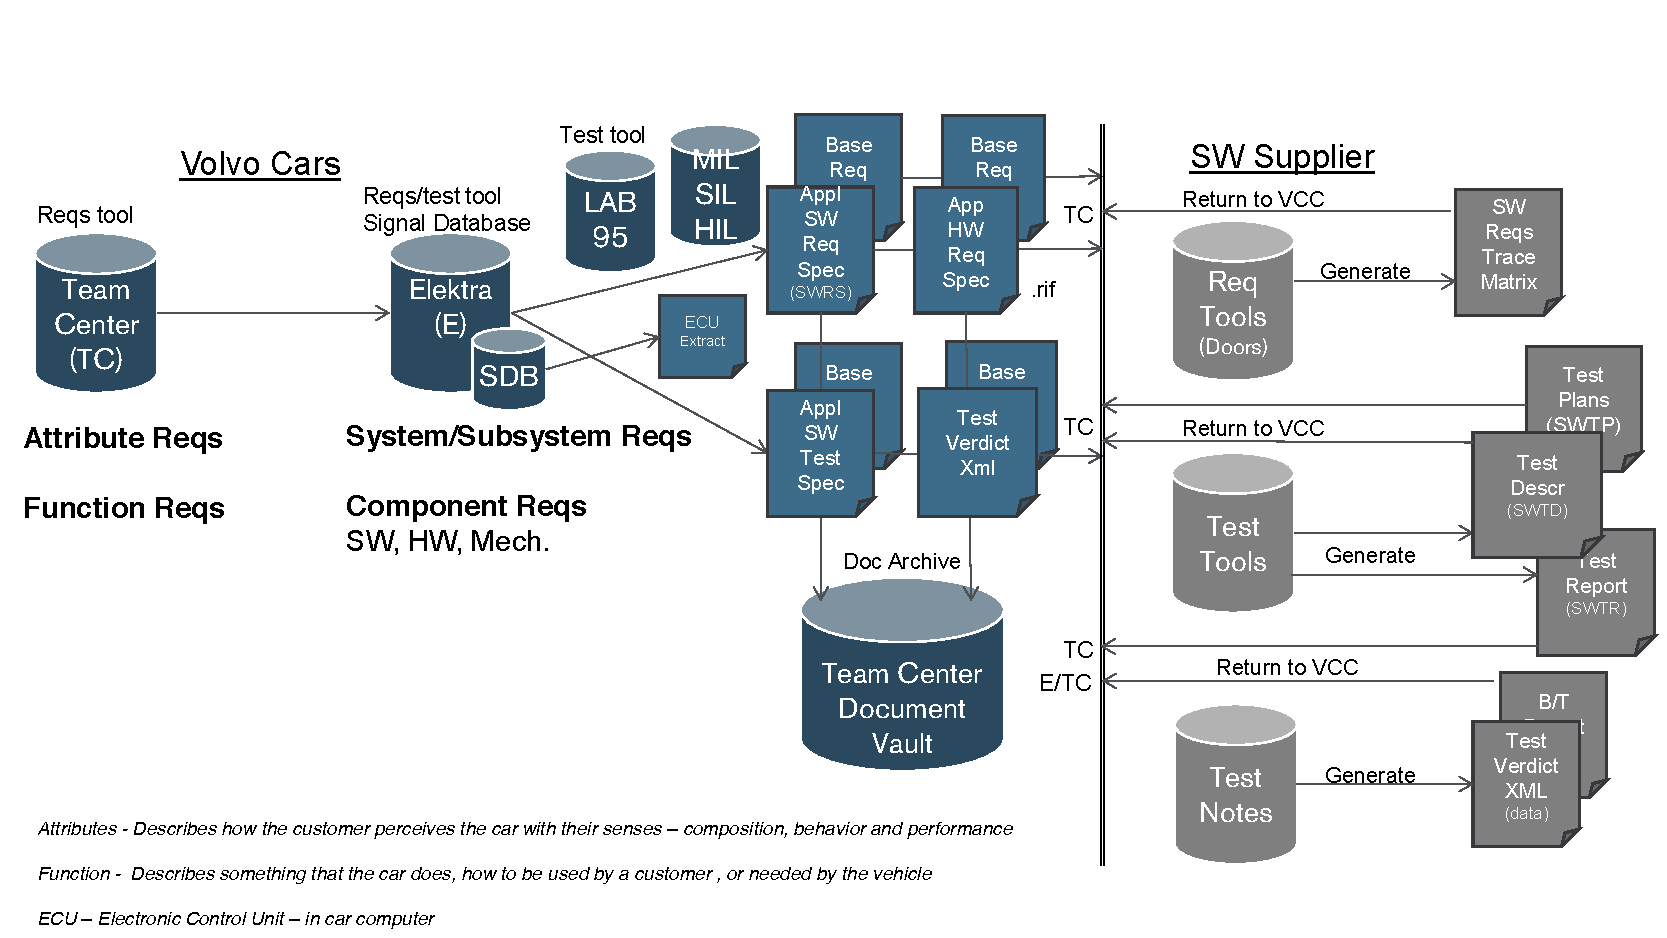
\includegraphics[width=0.95\linewidth]{figure/literatures/niesel_elektra.pdf}
\caption{Diagram showing the tool \textit{Elektra} treated as a database \cite{Niesel}}
\label{fig:niesel-elektra}
\end{figure}

To understand how Elektra has been used in development process, we arranged a meeting with Håkan Dahlen, a Software Developer who works with Central Electronic Module (CEM) which is one of the biggest and important ECUs within a car. In the meeting he  explained that searching for an artifact in Elektra was challenging because of the lack of visualization features in the tool. One of the examples that gives us a good explanation of the problem is, there was a problem with an LC where a fault signal from a port of one of its associated LCs was sent to. To solve the problem the in-house developers responsible for this component must look for the port using a search function in Elektra. The tool then returned a list of more than 20 ports of the associated LCs, which the developers had to check them one by one unless they knew by experience already which port was they were looking for. Thus, having a visualization of the signals sent/received among LCs would be an advantage in this aspect. \\

\section{Model-Driven Software Engineering}
A model has been defined by Czarnecki and Helsen ~\cite{Czarnecki} as it is an abstraction of a system and/or its environment. Models help to address questions that stakeholders may need in their work, it could be to provide a better understanding of the system which can aid in decision making.\\


In software development, models are used to depict software artifacts in software engineering activities throughout software development life cycle. A model itself is used as primary artifact representing more abstract view of a software to be built. In this context, this methodology is known as \textit{Model-Driven Software Engineering} (MDSE), aiming for tackling the complexity problem caused by the larger size of a software due to the needs of humans \cite{Brambilla}. The goals of MDSE also include increasing the software development speed which can be done by transformations (will be described later), reducing cost in long-term, and supporting the reuse of model for repeatable processes. \\

Based on the book \textit{`Allgemeine Modelltheorie (General Model Theory)'} written by Stachowiak \cite{Stachowiak}\footnote{ \url{https://modelpractice.wordpress.com/2012/07/04/model-stachowiak/} (english translation)}. He describes that a model should have 3 fundamental properties: \textit{reduction}, \textit{mapping}, and \textit{pragmatic}. Reduction property of a model is that it contains only details relevant to model creators and users. Generally speaking, the model does not include all details of its original. The mapping property means a model is always the model of something else i.e. its original. The pragmatic property of a model is the model can replace its original with respect to some purpose.

\begin{equation}
Models + Transformations = Software
\label{eg:mde}
\end{equation}

\subsection{Modeling languages}
\label{sec:modeling_languages}
Similar to Wirth equation, models and transformations need to be defined in some notation which in MDSE context it is called \textit{modeling languages}. A modeling language is a tool that designers use for specifying definition of the concrete representation of a model for a software system \cite{Brambilla}. It comprises of three main ingredients: \textit{abstract syntax}, \textit{concrete syntax}, and \textit{semantics} (see figure~\ref{fig:brambilla-modeling}). \\

\begin{figure}[H]
\centering
\captionsetup{justification=centering}
\vspace{0cm}% Adjust vertical spacing here
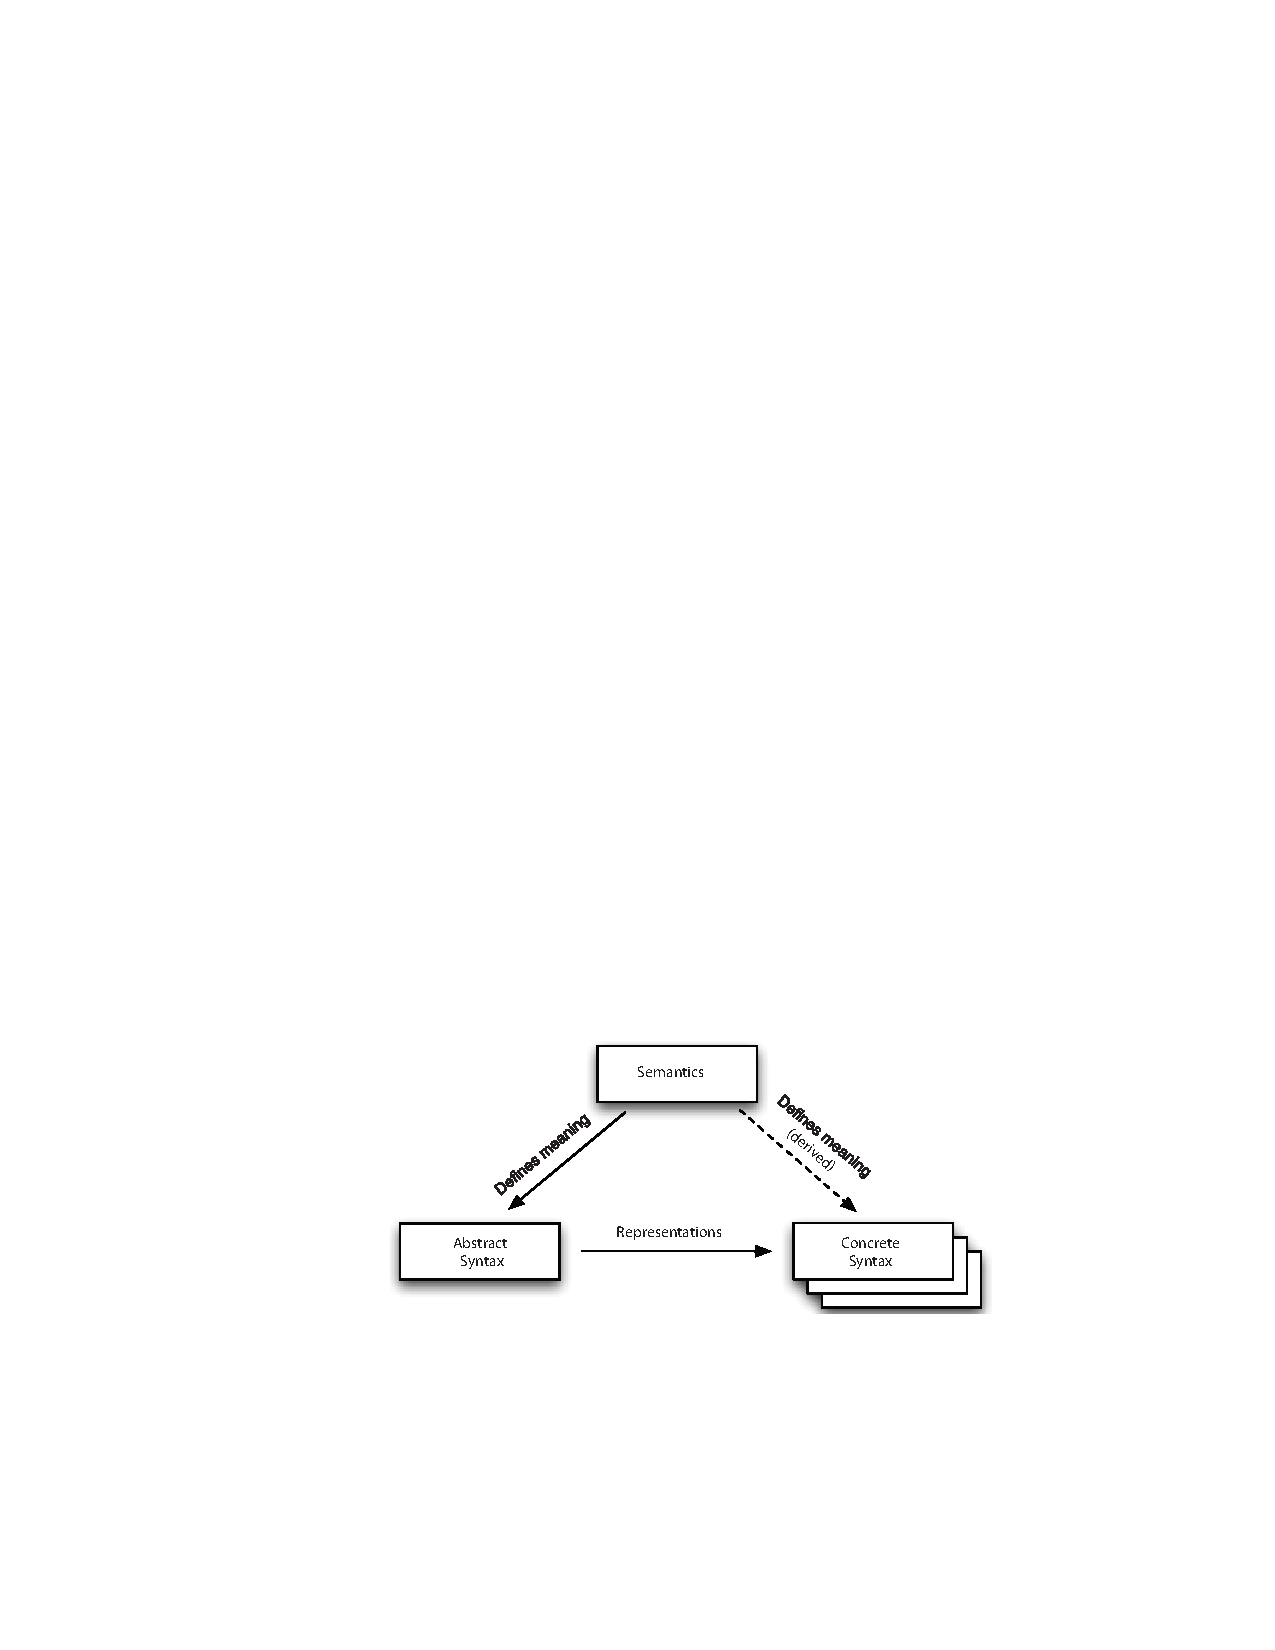
\includegraphics[width=0.6\linewidth]{figure/literatures/brambilla_modeling.pdf}
\caption{Three main ingredients that comprise a modeling language \cite{Brambilla}}
\label{fig:brambilla-modeling}
\end{figure}

A modeling language may consist of either graphical representations or textual representations, or both. Modeling languages can be classified into two main categories: Domain-Specific Language (DSL) and General-Purpose Modeling Language (GPML, GML, or GPL). DSLs are the languages that are designed for specific domain, context, or company. The purpose of this type of languages is to help people to describe and explain things in a certain domain. In contrast, GPLs are the languages that are designed for general use. They lack of specific features for a specific domain. An example of this type of languages is UML. \\

\subsubsection{Meta-models, model instances, and semantics}
As introduced in Section \ref{sec:modeling_languages}, The modeling languages comprises of three main ingredients: \textit{abstract syntax}, \textit{concrete syntax}, and \textit{semantics} (see figure~\ref{fig:brambilla-modeling}). An abstract syntax is defined using \textit{meta-models} \cite{Brambilla}. A meta-model is a precise definition of the parts and rules needed to create valid models \cite{Tichy}, so to speak a type of model used to describe the model.

\begin{figure}[H]
\centering
\captionsetup{justification=centering}
\vspace{0cm}% Adjust vertical spacing here
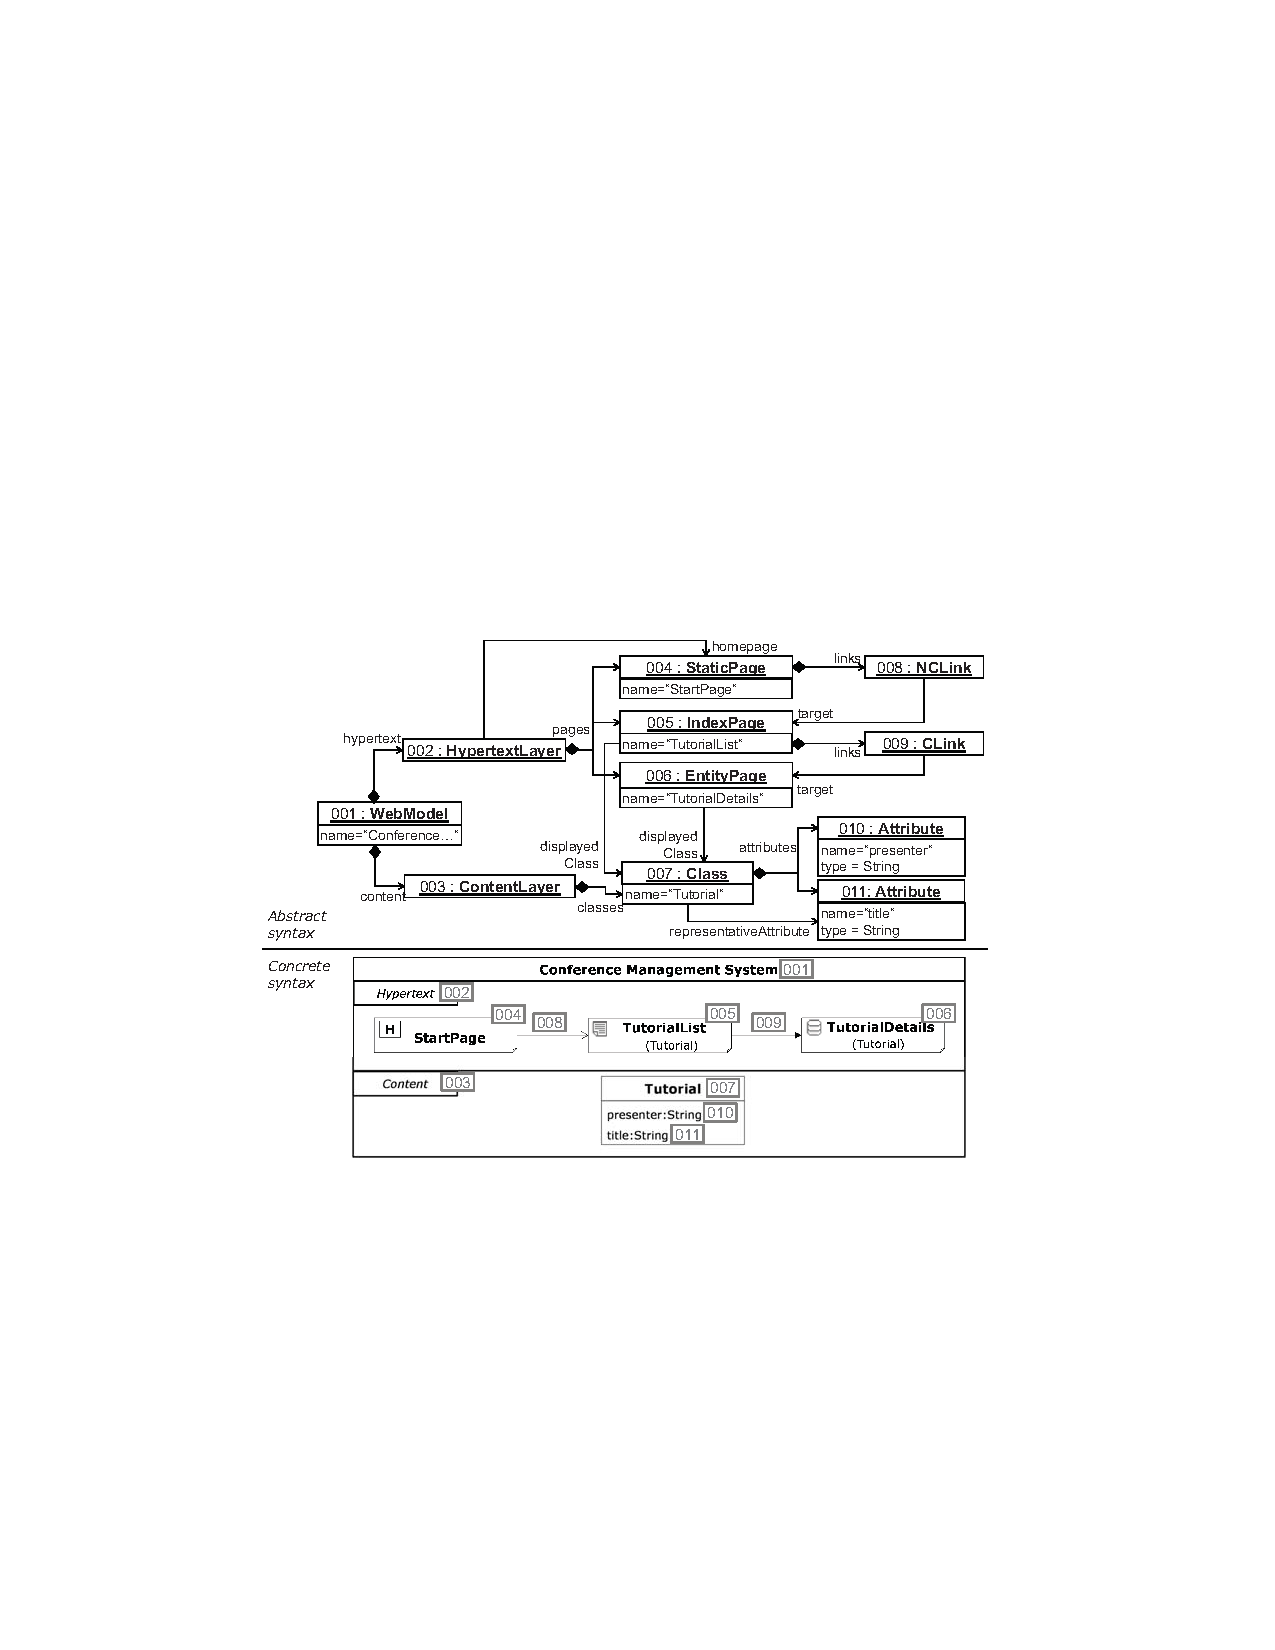
\includegraphics[width=0.75\linewidth]{figure/literatures/brambilla_abstract_concrete.pdf}
\caption{sWML model's abstract syntax and graphical concrete syntax \cite{Brambilla}}
\label{fig:brambilla-abstract-concrete}
\end{figure}

A concrete syntax is the concrete notation of a modeling language. It can be either a graphical or textual representation of \textit{model instances}. The figure~\ref{fig:brambilla-abstract-concrete} shows the abstract syntax and graphical concrete syntax of one of the well-known DSLs, simple Web Modeling Language (sWML). \\

The third ingredient of a modeling language is semantics. They define the meaning of abstract syntax and concrete syntax (indirectly). In software engineering, semantics are classified into two main categories: \textit{static semantics} and \textit{dynamic semantics}. The former specifies the allowed structure in a modeling language such as well-formedness and typing of meta-models, while the latter describes the execution behavior or run-time effect of a model \cite{Stuurman}.\\

In an integrated development environment (IDE), such as Eclipse\footnote{\url{https://eclipse.org/}}, you can create a meta-model and a model instance by using Eclipse Modeling Framework (EMF) with an Eclipse plug-in called \textit{EcoreTools}\footnote{\url{http://www.eclipse.org/ecoretools/}}. EcoreTools is a complete environment including a Graphical Ecore Editor (Figure~\ref{fig:screenshot_ecore_editor}) for creating meta-models (Ecore) and model instances. 

\begin{figure}[H]
\centering
\captionsetup{justification=centering}
\vspace{0cm}% Adjust vertical spacing here
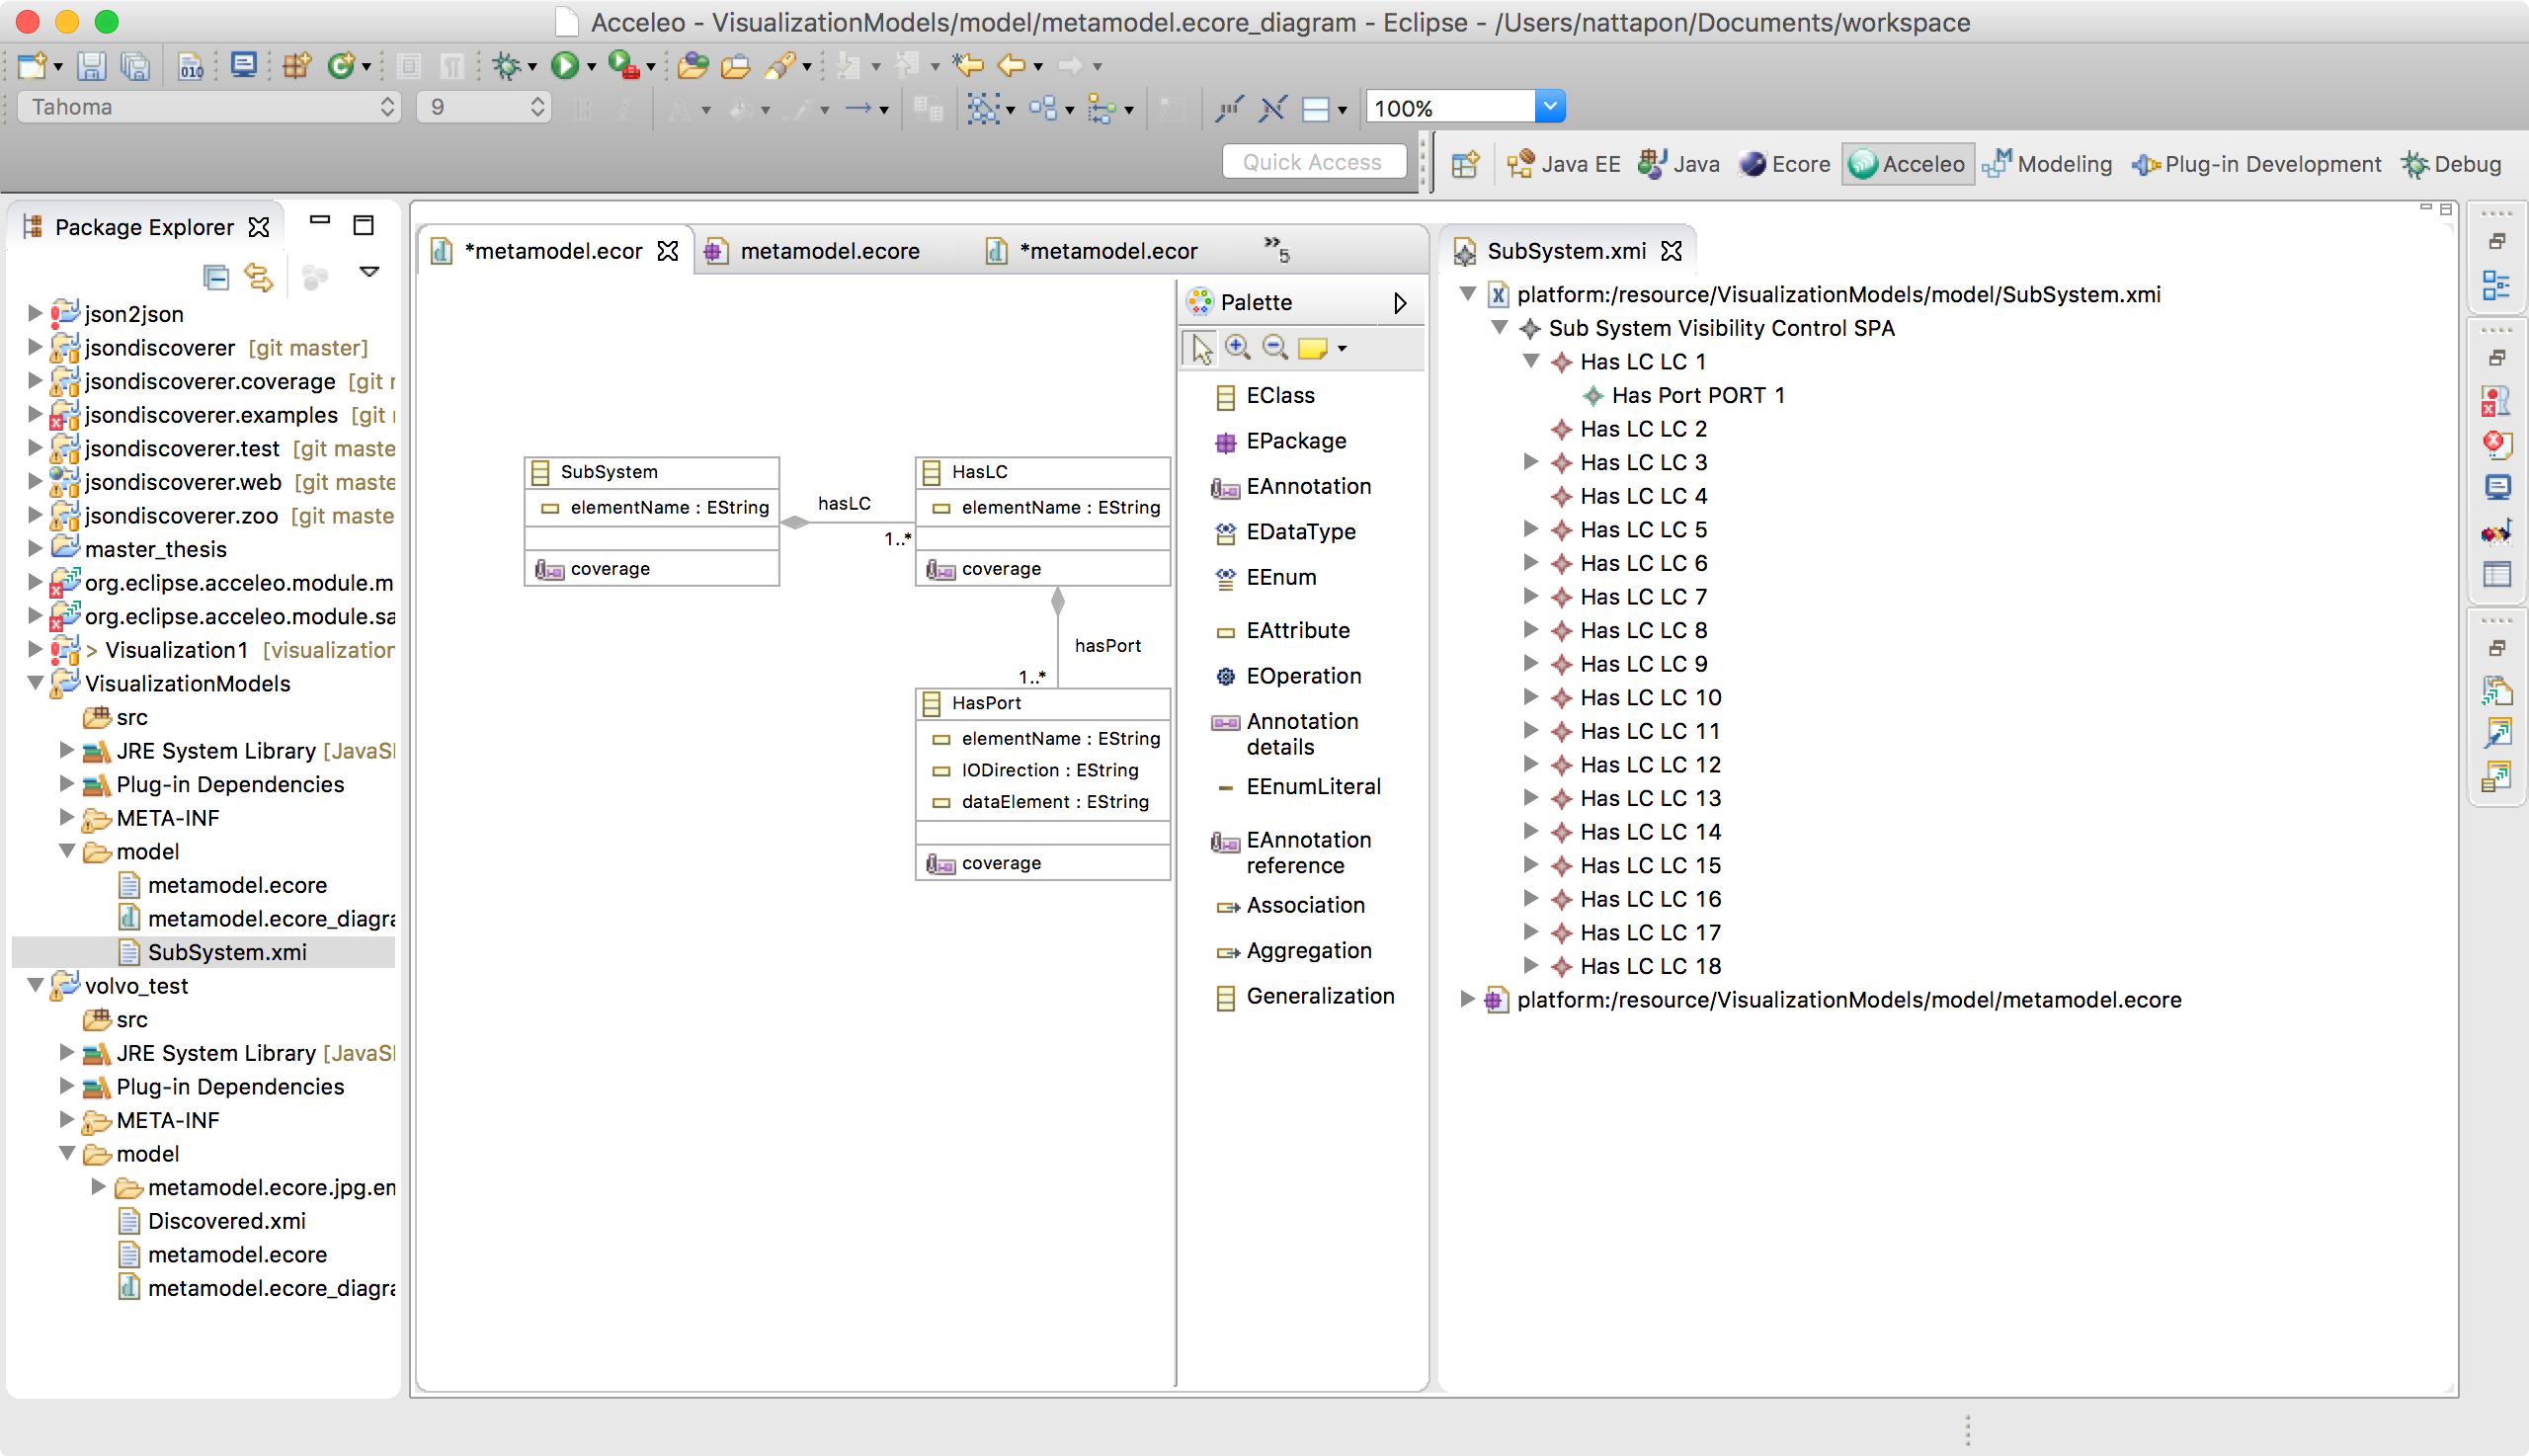
\includegraphics[width=0.95\linewidth]{figure/misc/screenshot_ecore_editor.png}
\caption{A screenshot of Graphical Ecore Editor in Eclipse}
\label{fig:screenshot_ecore_editor}
\end{figure}

An alternative way of creating a meta-model and a model instance is to use \textit{JSON discoverer}\footnote{\url{http://som-research.uoc.edu/tools/jsonDiscoverer/}}. JSON discoverer is an open-source project developed by Javier Luis Cánovas Izquierdo and Jordi Cabot. It provide a feature that automatically discovers the implicit schema (meta-model) and a data model (mdoel instance) of a set of JSON file. This means a set of data in JSON format is required. \\ 

In our case, choosing JSON discoverer tool is a good practice since data in Elektra can be extracted in JSON format. To create a meta-model and the model instance, we simply import the JSON file as an input to the tool. An explaination of how to do so will be discussed in Chapter~\ref{methodology}.


\subsection{Model transformation}
Model transformation is another core concept of MDSE as seen in the equation \ref{eg:mde} proposed by Stachowiak which is based on Niklaus Wirth famous equation\footnote{For further discussion, see Wirth, N. (1976). \textit{Algorithms + data structures=programs}. Englewood Cliffs, N.J.: Prentice-Hall.}. It allows the mappings between different models. An example of transformation is transforming UML class diagram\footnote{A static structure diagram that represents the structure of a system showing classes, attributes, methods, and the relations among objects.} to Entity-relationship (ER) diagram\footnote{A data model that describes data in business aspect.}.

\begin{figure}[H]
\centering
\captionsetup{justification=centering}
\vspace{0cm}% Adjust vertical spacing here
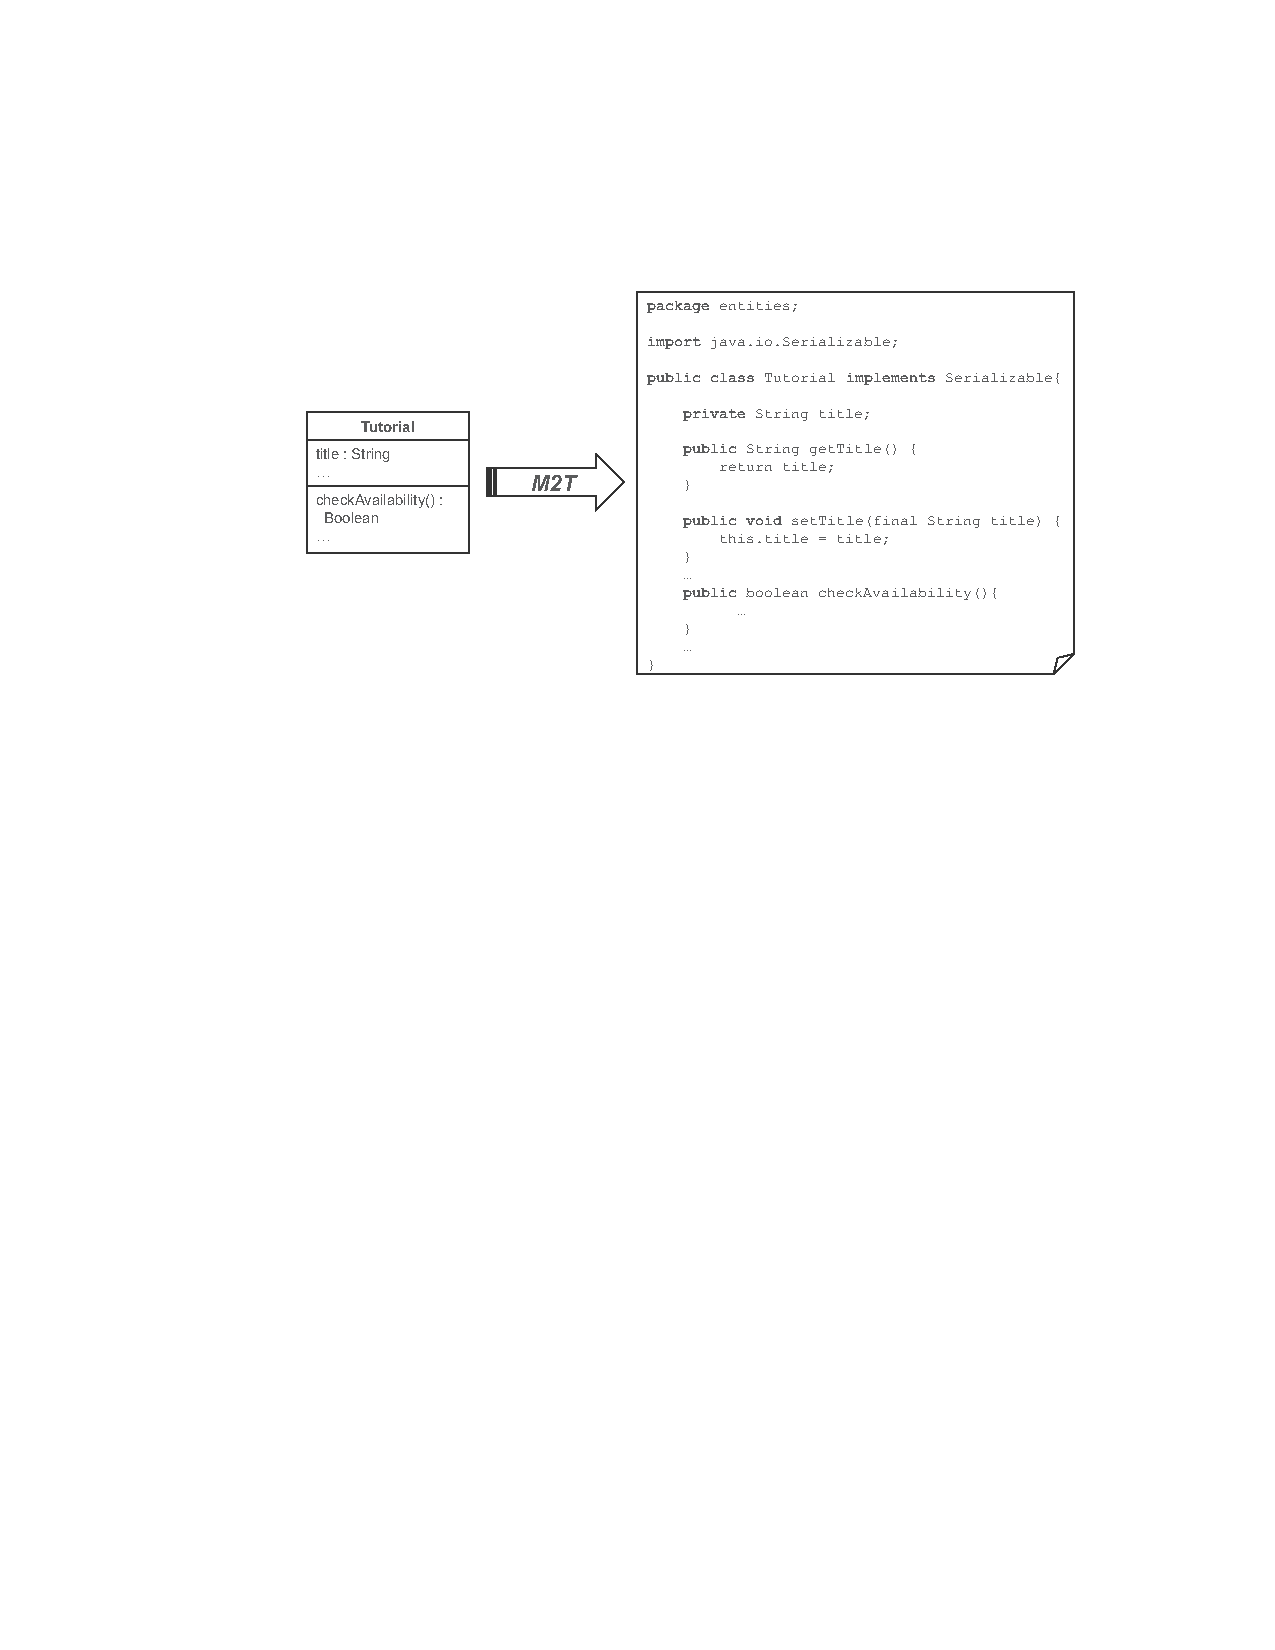
\includegraphics[width=0.8\linewidth]{figure/literatures/brambilla_m2t_example.pdf}
\caption{An example of M2T transformation~\cite{Brambilla}}
\label{fig:brambilla-m2t}
\end{figure}

There are two kinds of model transformation, model-to-model (M2M) and model-to-text (M2T) transformation. M2M transformation takes in a source model as the input and the output is named a target model. The target result of M2T transformation is just a strings. The model transformation can be done by using  template-based approach or visitor-based approach \cite{Czarnecki}. In this report, we are mostly interested with M2T transformation and we have applied template-based approach. A number of template engines are available to do a M2T transformation. In this thesis work we use \textit{Acceleo}\footnote{\url{https://eclipse.org/acceleo/}} as the main engine. The template engines are capable of generating files with texts of different formats depending on how the generator file has been programed. The content of a generated file(s) depends on the meta-model specified and also the model instance of a meta-model. An example of M2T transformation can be seen in Figure~\ref{fig:brambilla-m2t}.

\section{Visualization of the architectures}
The output from M2T transformation is textual description. It is used for generating visualization based on a model instance, which conforms to its meta-model. To create a visualization of the electrical architectures, several tools such as PlantUML\footnote{\url{http://plantuml.com/}} and Umple\footnote{\url{http://cruise.eecs.uottawa.ca/umple/}} can be used. In this thesis work, we choose PlantUML as a main visualization tool. PlantUML is an open-source project developed by Arnaud Roques. The tool allows users to create UML diagrams from textual description written in its DSL. The language of PlantUML is well-formed and human-readable code from which the diagrams are rendered.

\begin{lstlisting}[caption=An example of textual description of a class diagram, label=code:plantuml_class]
@startuml

class Accommodation {
  +Int Floor
  +Int Wall
  +Int Ceiling
  +Int Door
  +Int Window
}

class Apartment
class House

Accommodation <|-left- Apartment: Inheritance
Accommodation <|-right- House: Inheritance

@enduml
\end{lstlisting}

\begin{figure}[H]
\centering
\captionsetup{justification=centering}
\vspace{0cm}% Adjust vertical spacing here
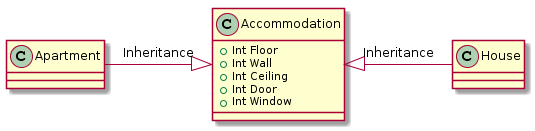
\includegraphics[width=0.8\linewidth]{figure/misc/plantuml_class.png}
\caption{UML class diagram rendered from the textual description in Listing~\ref{code:plantuml_class}}
\label{fig:plantuml_class}
\end{figure}

Different types of UML diagrams such as class diagrams can be generated. Figure~\ref{fig:plantuml_class} shows the UML class diagram rendered from the code in Listing~\ref{code:plantuml_class}.\\

UML component diagrams can also be created from the textual description by using some specific syntax shown in the table~\ref{table:plantuml_component_syntax}. The use of the syntax will be explained in Chapter~\ref{methodology}. 

%\begin{table}[H]
%\centering
%\renewcommand{\arraystretch}{1.5}% Spread rows out...
\begin{longtable}{>{\centering}m{1.8in} >{\centering}m{2in} >{\centering\arraybackslash}m{1.5in}}
\toprule
\textbf{Description} & \textbf{PlantUML syntax} & \textbf{Representation} \\
\midrule
Artifact & \texttt{artifact artifact1} & 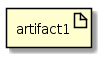
\includegraphics[width=0.45\linewidth]{figure/plantuml_example/artifact.png} \\ \hline
Component & \texttt{[component]} & 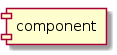
\includegraphics[width=0.6\linewidth]{figure/plantuml_example/component.png} \\ \hline
Components, ports, and connection &  \texttt{[c1] \#-\# [c2]} & 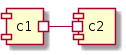
\includegraphics[width=0.7\linewidth]{figure/plantuml_example/port.png}\\ \hline
Components, required/provided ports, and connection & \texttt{[c1] \#-(0-\# [c2]} & 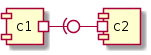
\includegraphics[width=0.8\linewidth]{figure/plantuml_example/port_type.png}\\
\bottomrule
\caption{Some useful syntax for UML component diagrams}
\label{table:plantuml_component_syntax}
\end{longtable}
%\end{table}

With the combination use of the syntax for UML component diagram, visualizing electrical architectures consisting of LCs and ports is possible.
%%%%%%


\section{Stakeholders}
On referring to the article of community tool box, there are three three different kinds of stakeholders : primary stakeholders, secondary stakeholders and key stakeholders. In this thesis, we interview different stakeholders during the phase II in methodology. Some of the advantages of interviewing the stakeholders include: getting more ideas, obtaining different perspectives, helps to avoid misunderstanding of the problem, and also increases the chances of delivering a valuable output to the stakeholders.\\

The primary stakeholders in our case are the people who are directly interacting with Elektra, also named beneficiaries and we, the students are the target. The act of visualization can aid the beneficiaries in obtaining a simplified overview of a data found in Elektra which in turn can provide a quick understanding of the needed artifacts and the interactions between these artifacts. \\

The secondary stakeholders are the ones who are indirectly affected by Elektra. They are the ones who may be affected by the decision made by the stakeholders who interacts directly with Elektra, which in turn will be due to the use of the obtained visualization. Our supervisors at the university can also be in a group of secondary stakeholders, they are not directly interacting with the obtained visualization but they also play a greater role in pushing forward our goals for delivering a good visualization. \\

The key stakeholders are the one funding this project and these can be the two supervisors from the company. All these stakeholders play a very important role in bringing efforts that could result to a better solution of the problem that we intend to resolve.\\

We, the students and as part of the primary stakeholders (targets), we intend to provide a visualization output that can aid in quick understanding of the data stored in Elektra and also provide the job opportunity for the need of having such a visualization tool to give the overview of the architecture. \\

%%%%%%

\section{Data collection method}
One of the key activities of this thesis work is to collect data from stakeholders. the team did some research and found a good method for data collection written by Basili and Weiss \cite{Basili}. The authors developed a goal-oriented data collection method for evaluating software development methodologies. The data that were used in the study were obtained from the changes in 5 software projects developed by different groups with different backgrounds using different development methodologies. They suggest 6 basic steps of data collection as follow:\\[0.1cm]

\begin{step} \label{step:1}
Establishing the goals of the data collection. What are the goals of performing data collection? Why is collecting data needed?
\end{step}

\begin{step} \label{step:2}
Developing a list of questions of interest. What kinds of questions that this study will answer corresponding to the goals in step \ref{step:1}?
\end{step}

\begin{step} \label{step:3}
Establishing data categories. Categories of data must be defined before collecting data.
\end{step}

\begin{step} \label{step:4}
Designing and testing data collection form. A form that is used to collect data must be created before collecting data.
\end{step}

\begin{step} \label{step:5}
Collecting and validating data. Data that are collected must be validated to ensure that they are accurate and complete.
\end{step}

\begin{step} \label{step:6}
Analysing data. Data are analyzed in order to answer the questions in step \ref{step:2}.
\end{step}

Basili and Weiss also suggest that validation of data is a key factor in data gathering. It must be done to ensure ensures correctness, consistency and completeness of data.